\chapter{Model Performance}
\label{chapter:ModelPerformance}

In this chapter the performance metrics of the best deep neural network model are described. The hyper-parameter values for the best model are enumerated in Section~\ref{sec:BestModel}.

\section{Training Metrics}
\label{sec:Training}

In Figure~\ref{fig:AccuracyLoss} the binary accuracy and loss function are presented. These result directly from training in Keras and Tensorflow. The Train dataset is balanced. While in general the Test dataset is unbalanced, for these plots Test is also balanced. This is done because it would be too slow to train the NN with 1200 epochs with Test unbalanced. Training is done on the balanced Train dataset. Prediction is done on the unbalanced Test dataset.

\begin{figure}[t]
\centering
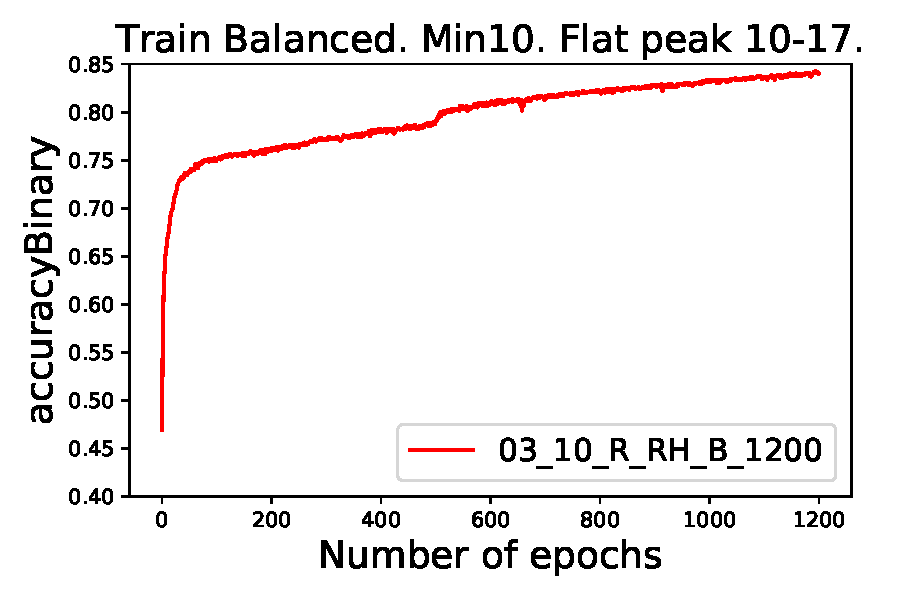
\includegraphics[width=0.45\textwidth]{plots/plot_01_1_overlay_graph_accuracyBinary_Train.pdf}
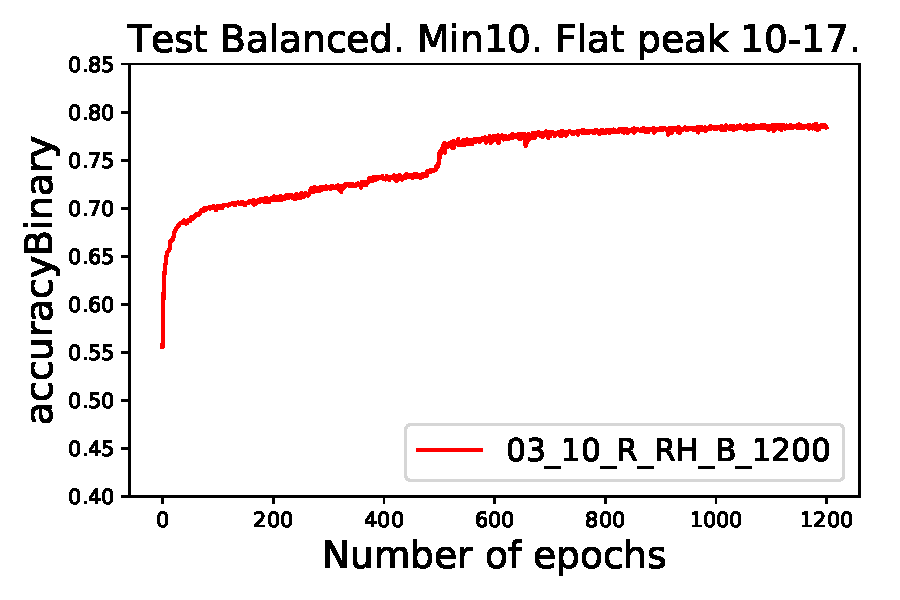
\includegraphics[width=0.45\textwidth]{plots/plot_01_1_overlay_graph_accuracyBinary_Test.pdf}\\
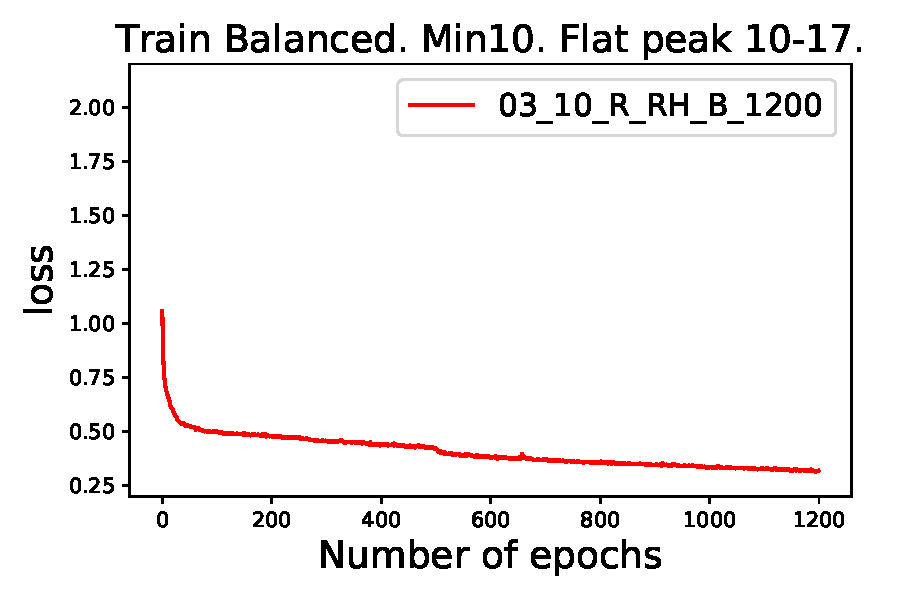
\includegraphics[width=0.45\textwidth]{plots/plot_01_1_overlay_graph_loss_Train.pdf}
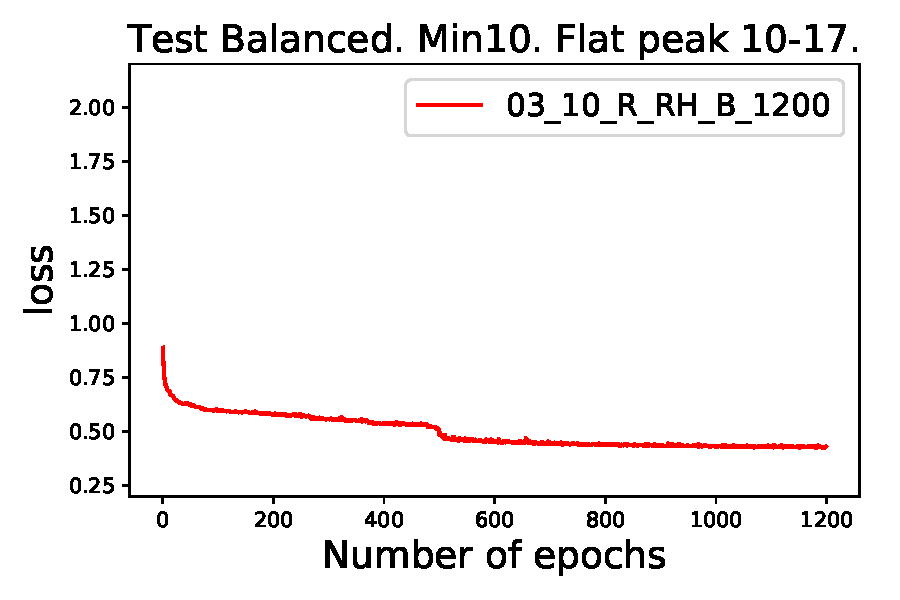
\includegraphics[width=0.45\textwidth]{plots/plot_01_1_overlay_graph_loss_Test.pdf}\\
\caption{Binary accuracy and loss, resulting directly from training in Keras and Tensorflow. Note that while Train is balanced, Test is also balanced, as it would be too slow to have it unbalanced.}
\label{fig:AccuracyLoss}
\end{figure}

\section{Hit-Level Metrics}
\label{sec:HitLevelMetrics}

In this section the metrics at the hit level are studied. A bucket is made of 20 hits. Figure~\ref{fig:OutputOutputPredicted1D} presents at the top the distribution of the number of positive hits ($\nbPositiveHit$), and at the bottom the distribution of the number of hits predicted to be positive, with Train on the left and Test on the right. The distributions are normalised, so their shapes can be compared. The number of events used in Train relative to Test is 7 to 3. Furthermore, the Train dataset is balanced, keeping only a subset of the buckets, while the Test dataset is unbalanced, keeping all of its buckets. In both datasets all values of $\nbPositiveHit < 10$ are set artificially to 0, effectively saying there is no hit belonging to an interesting particle in this bucket. Furthermore, the Train dataset is balanced, so that some of the buckets with $\nbPositiveHit$ between 10 and 17 are eliminated, so that equal numbers of buckets for each \nbPositiveHit~remain. Since the distribution is falling (as seen in the Test plot), all values take the lower value of bin 17.

\ \\Tests were done with values flattened from 10 to 14, through 10 to 20. Ending the interval lower than 17 would not have a training distribution flat enough. Ending the interval higher than 17 would leave very few buckets to train on. Therefore values for bins 18-20 are left unchanged, as they are too small.

\ \\At the bottom of Figure~\ref{fig:OutputOutputPredicted1D} there are the equivalent plots after prediction using our model. Comparing the actual values on top with the predicted values at the bottom, the same features in the plots are observed. There is a tall bin at $\nbPositiveHit = 0$, followed by nearly empty bins. Then the distributions starts to grow at $\nbPositiveHit = 10$, just as in the desired output distribution. For the higher bins, the relative shape does not agree fully to the desired output. For Train, instead of being flat, the distribution increases with larger \nbPositiveHit. For Test, the distribution decreases as expected, but not nearly as fast. Overall, however, the model behaves quite well, relative to many other hyper-parameter settings tried.

\begin{figure}[t]
\centering
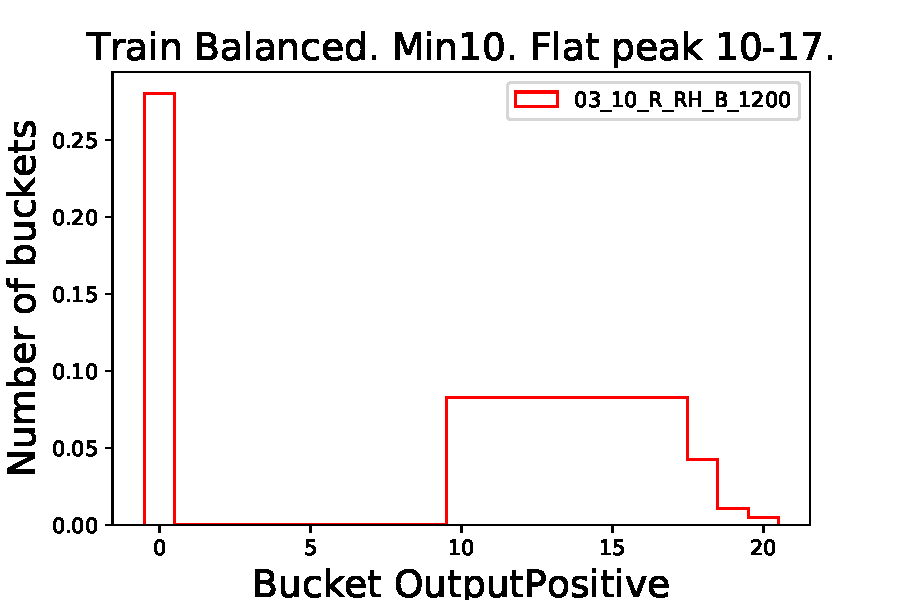
\includegraphics[width=0.45\textwidth]{plots/plot_02_1_overlay_histo_OutputPositive_Train.pdf}
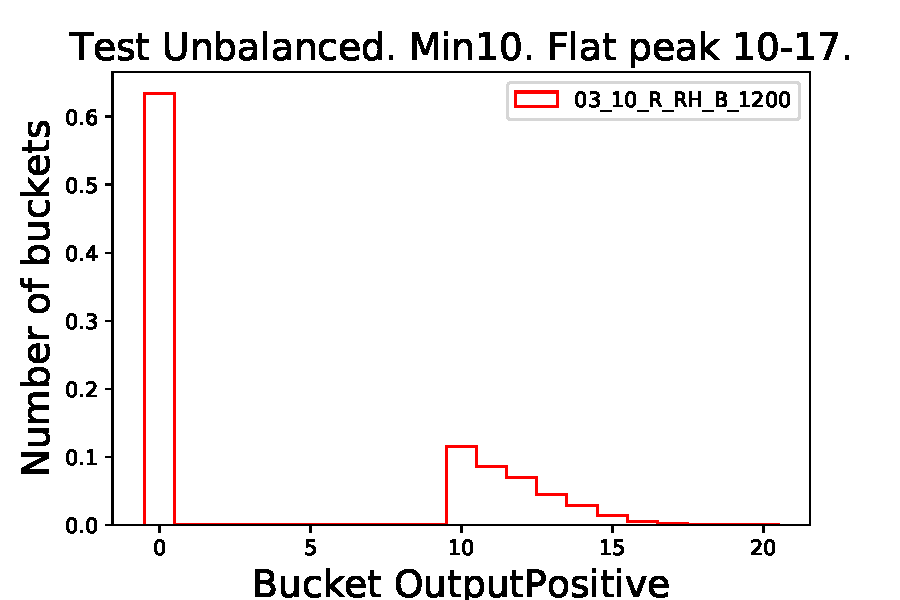
\includegraphics[width=0.45\textwidth]{plots/plot_02_1_overlay_histo_OutputPositive_Test.pdf}\\
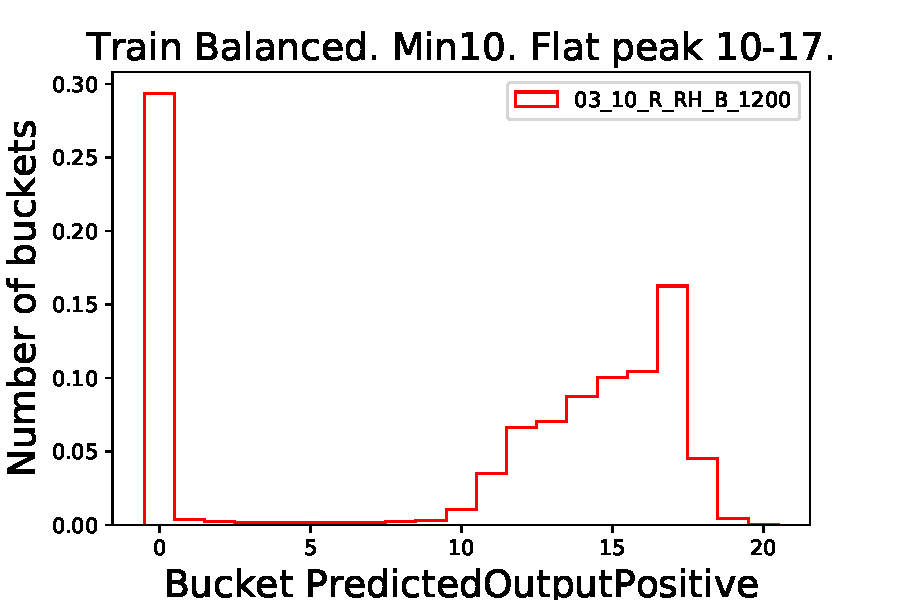
\includegraphics[width=0.45\textwidth]{plots/plot_02_1_overlay_histo_PredictedOutputPositive_Train.pdf}
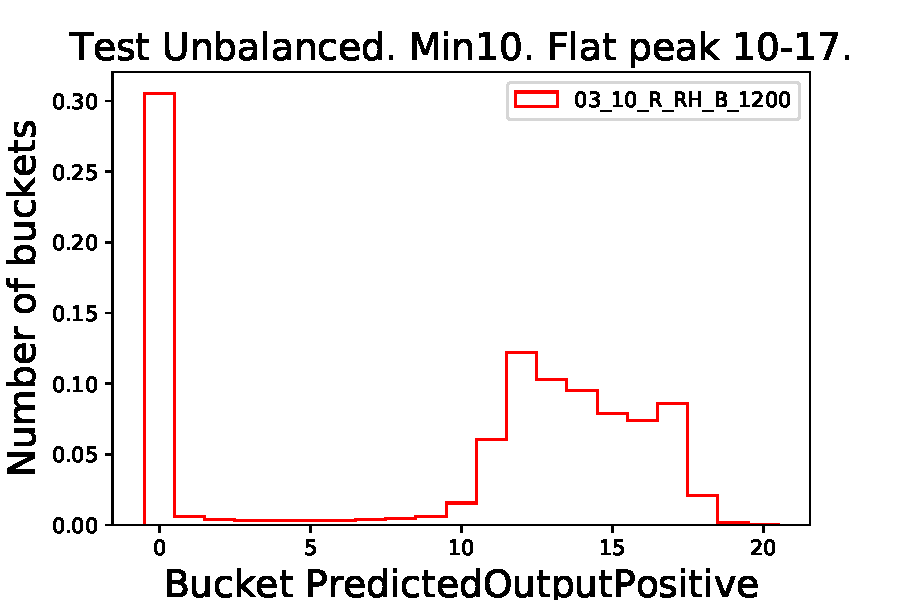
\includegraphics[width=0.45\textwidth]{plots/plot_02_1_overlay_histo_PredictedOutputPositive_Test.pdf}\\
\caption{Output and output predicted 1D}
\label{fig:OutputOutputPredicted1D}
\end{figure}

\ \\Figure~\ref{fig:OutputOutputPredicted2D} presents the 2D distributions of the output predicted vs output in terms of the number of positive hits. The colour coding is proportional to the number of entries in the 2D histogram. As expected, there is a peak at (0, 0). These events have exactly zero number of positive hits (after moving all values smaller than 10 to 0), and are also predicted to have exactly zero number of positive hits. There is nothing between 1 and 9. And for values $\ge 10$, there is a diagonal for the Train balanced. When the training is accurate, a diagonal is expected because the predicted output will be similar to the actual output. For the Test unbalanced, the diagonal is harder to see. But indeed most entries are in the top left corner of this region, as expected.

\begin{figure}[t]
\centering
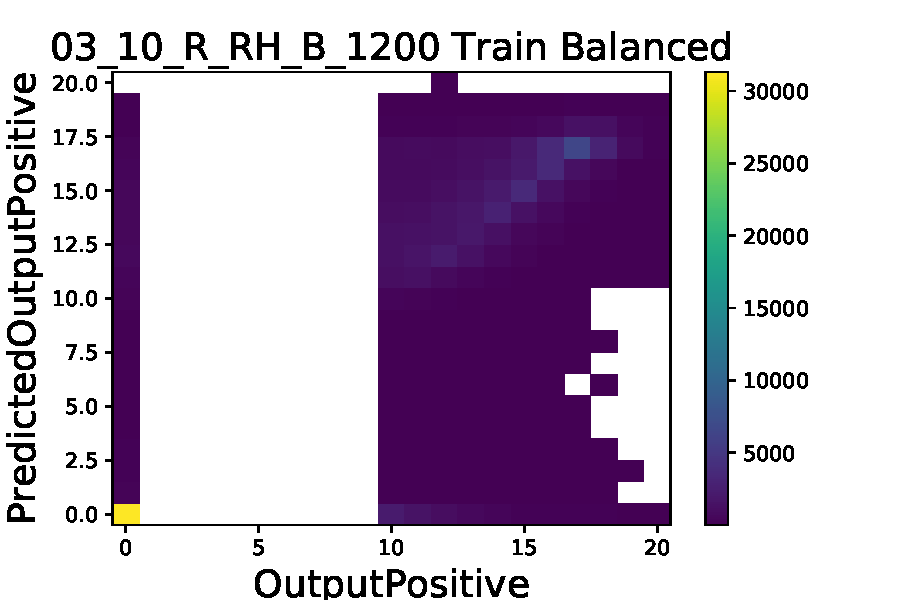
\includegraphics[width=0.45\textwidth]{plots/plot_04_1_overlay_histo2D_OutputPositive_PredictedOutputPositive_03_10_R_RH_B_1200_Train.pdf}
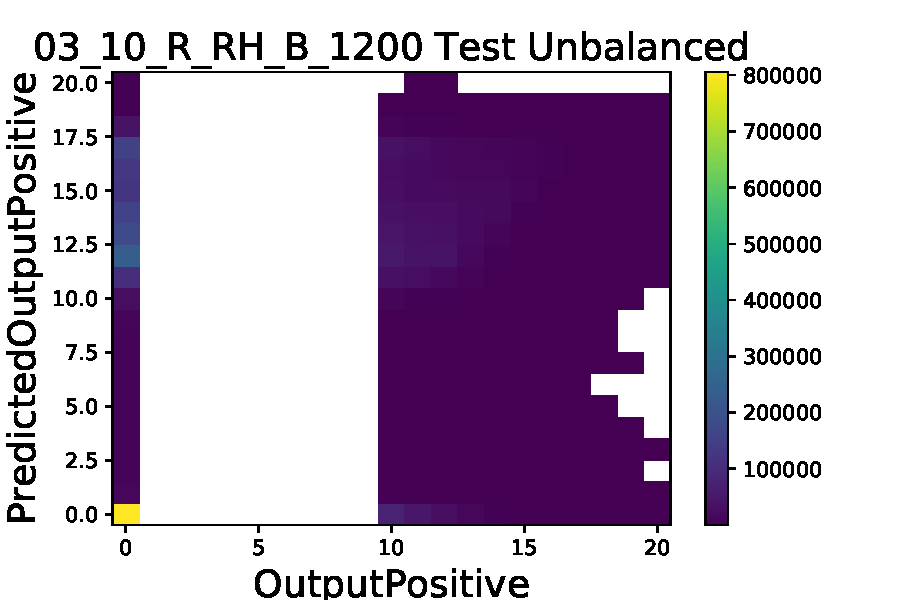
\includegraphics[width=0.45\textwidth]{plots/plot_04_1_overlay_histo2D_OutputPositive_PredictedOutputPositive_03_10_R_RH_B_1200_Test.pdf}\\
\caption{Output and output predicted 2D. In Train balanced, a diagonal is seen. In Test unbalanced, it's harder to see.}
\label{fig:OutputOutputPredicted2D}
\end{figure}

\ \\From these plots it can be concluded that in the balanced dataset (Train and Test) a diagonal can be seen. In the Test unbalanced it is harder to see, but values still look relatively flat in 1D. 

\ \\Figure~\ref{fig:FiguresOfMerit1} presents figures of merit at hit level for each \volumeID~in the detector. By looping over all buckets and all hits, both the true and predicted output labels for each hit are known. Each hit prediction can be either TP (True Positive), FP (False Positive), FN (False Negative), or TN (True Negative). The number of hits in these four categories in each \volumeID~is counted. From these, for each \volumeID~several figures of merit are estimated: accuracy, precision, recall, predicted output negative and true negative rate. They all need to be as high as possible, ideally 1.0. As is known from the bias-variance trade-off, it is impossible for any model to satisfy all criteria. For this reason, a model with overall good performance across all categories is chosen.

\begin{figure}[t]
\centering
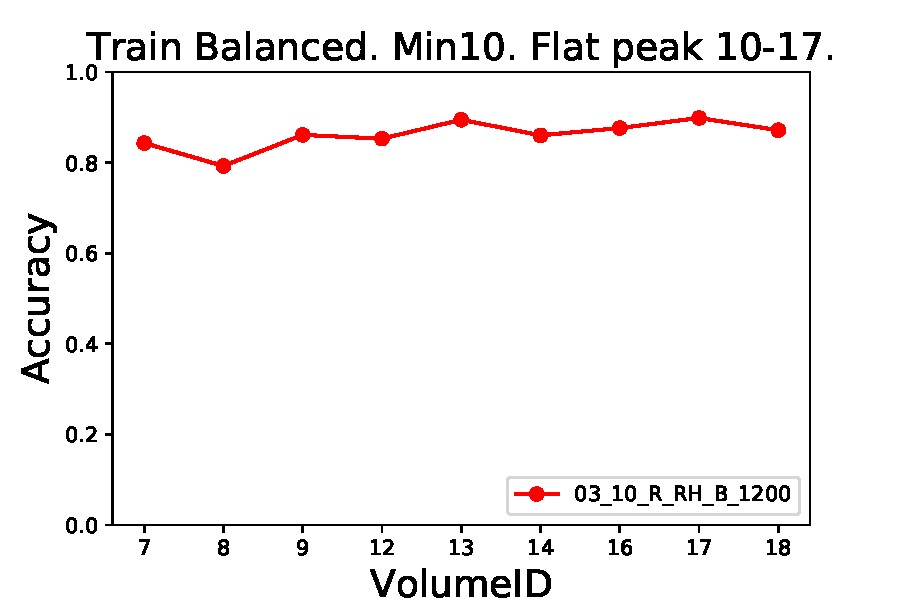
\includegraphics[width=0.45\textwidth]{plots/plot_03_1_overlay_graph_Accuracy_VolumeID_Train.pdf}
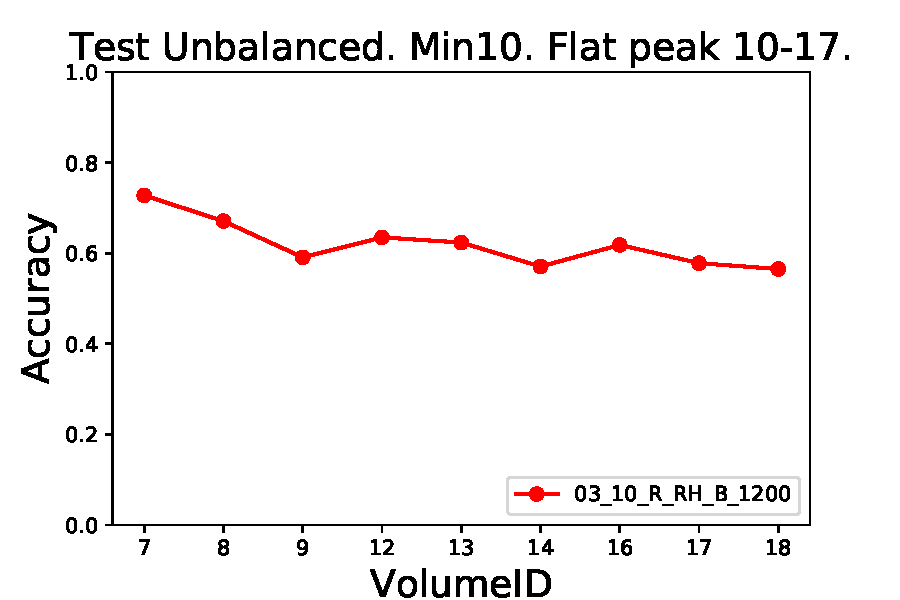
\includegraphics[width=0.45\textwidth]{plots/plot_03_1_overlay_graph_Accuracy_VolumeID_Test.pdf}\\
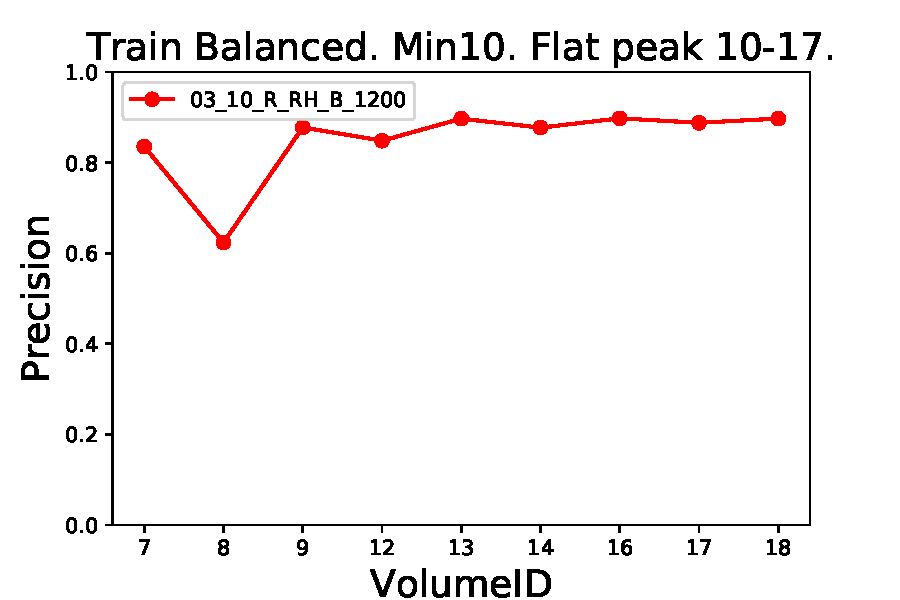
\includegraphics[width=0.45\textwidth]{plots/plot_03_1_overlay_graph_Precision_VolumeID_Train.pdf}
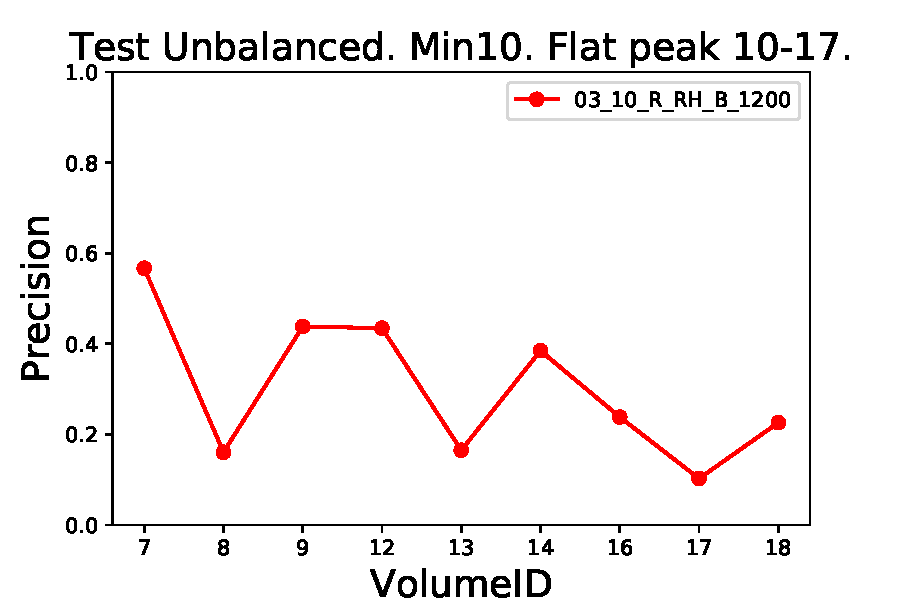
\includegraphics[width=0.45\textwidth]{plots/plot_03_1_overlay_graph_Precision_VolumeID_Test.pdf}\\
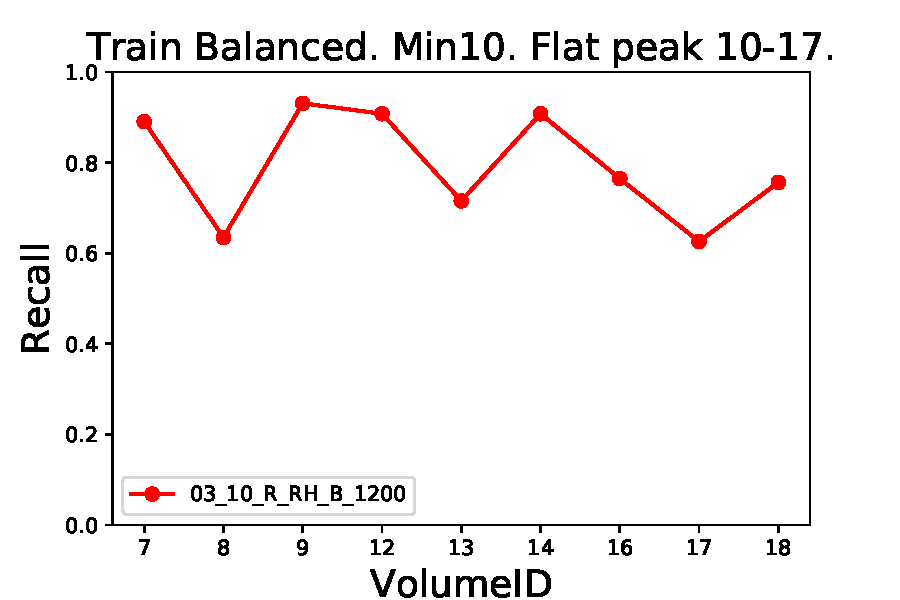
\includegraphics[width=0.45\textwidth]{plots/plot_03_1_overlay_graph_Recall_VolumeID_Train.pdf}
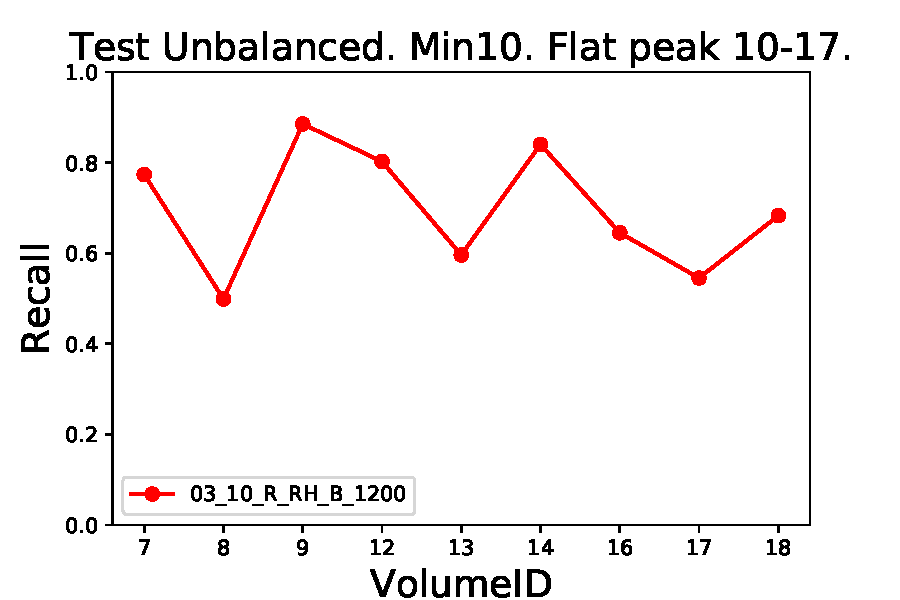
\includegraphics[width=0.45\textwidth]{plots/plot_03_1_overlay_graph_Recall_VolumeID_Test.pdf}\\
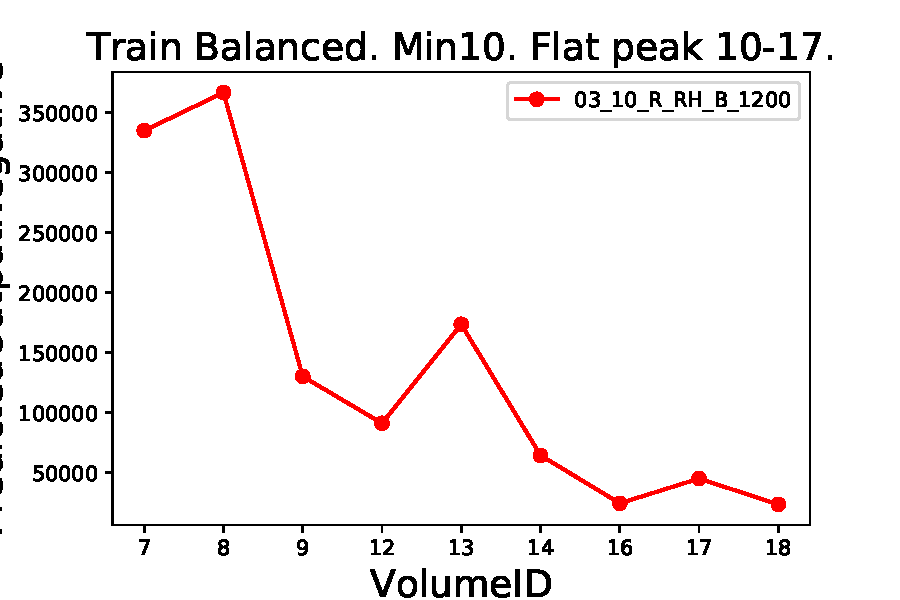
\includegraphics[width=0.45\textwidth]{plots/plot_03_1_overlay_graph_PredictedOutputNegative_VolumeID_Train.pdf}
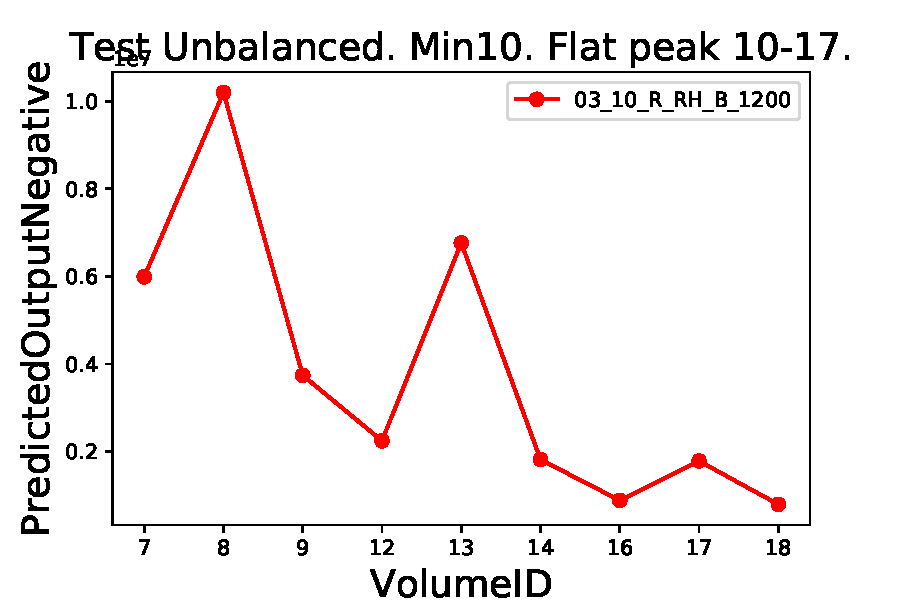
\includegraphics[width=0.45\textwidth]{plots/plot_03_1_overlay_graph_PredictedOutputNegative_VolumeID_Test.pdf}\\
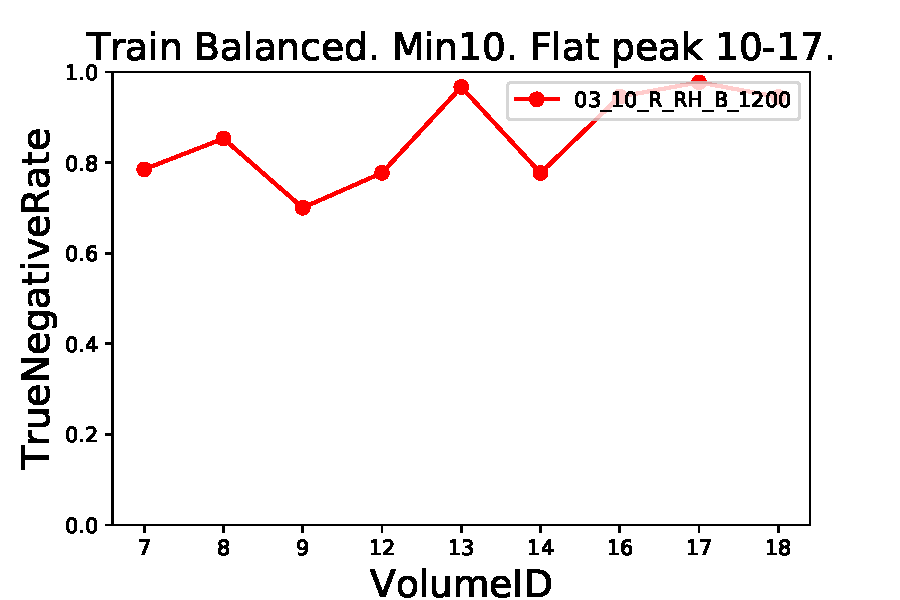
\includegraphics[width=0.45\textwidth]{plots/plot_03_1_overlay_graph_TrueNegativeRate_VolumeID_Train.pdf}
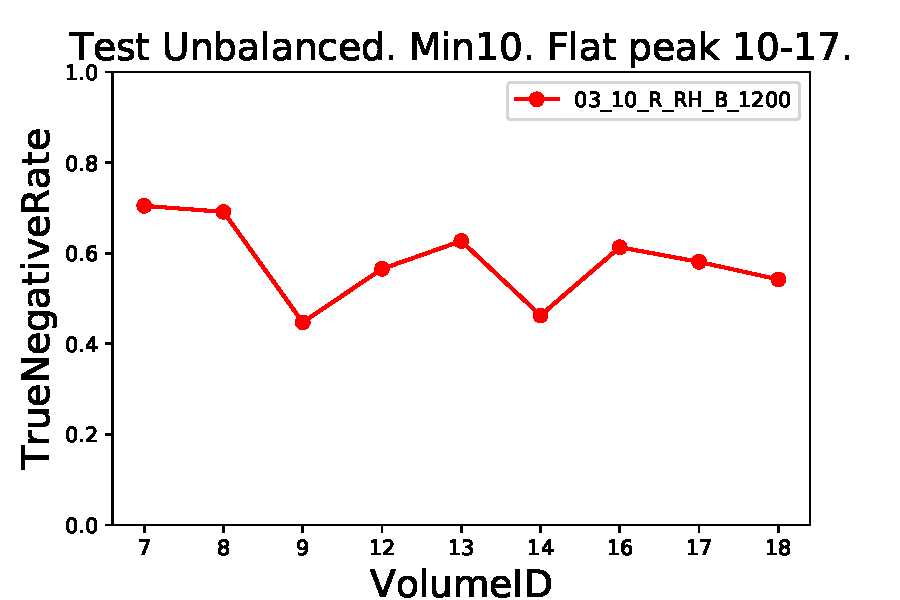
\includegraphics[width=0.45\textwidth]{plots/plot_03_1_overlay_graph_TrueNegativeRate_VolumeID_Test.pdf}\\
\caption{Accuracy, precision, recall, predicted output negative, true negative rate. Train (left) and Test (right).}
\label{fig:FiguresOfMerit1}
\end{figure}

\section{Particle-Level Metrics}
\label{sec:ParticleLevelMetrics}

Two numpy arrays of dimension two are used: the true output and the output predicted by the model. Each row represents a bucket. There are 20 columns, representing the 20 hits in the bucket. A for loop over buckets is made. For each bucket a loop over hits is made. Each hit has a value of -1 or +1 for the output and for the predicted output. For the current bucket, the number of hits that are positive (\nbPositiveHit) is counted. A count is also made for those that are both positive and in addition predicted to also be positive (\nbTruePositiveHit). A bucket with $\nbPositiveHit \ge 10$ is considered to contain a truth particle. If in addition the bucket also has $\nbTruePositiveHit /\nbPositiveHit > 80\%$, it is also considered to have reconstructed that particle correctly. A count is made of the buckets that have a truth particle. Then a separate count is made of those buckets that have a truth particle, and in addition has reconstructed the truth particle. The efficiency of reconstructing a particle ($\eff = \nbParticleReco / \nbParticleTruth$) is 84.2\% for Train and 71.3\% for Test. Detailed results are summarised in Table~\ref{tab:ParticleReconstructionEfficiency}.

\begin{table}[h!]
\centering
  \resizebox{\textwidth}{!}{
    \begin{tabular}{|l|l|l|l|l|} % <-- Alignments: 1st column left, 2nd middle and 3rd right, with vertical lines in between
      \hline
      Sample & \eff & \nbBucket & \nbParticleTruth & \nbParticleReco \\
      \hline
      Train Balanced & 84.2\% & 130k & 94k & 79k \\
      Test Balanced & 74.9\%  & 62k & 45k & 34k \\
      Test Unbalanced & 71.3\% & 3219k & 1178k & 840k \\
      \hline
    \end{tabular}
  }
\caption {Particle reconstruction efficiency results}
\label{tab:ParticleReconstructionEfficiency}
\end{table}
